\documentclass[11pt]{article}
\usepackage{classTools}

\begin{document}

\psHeader{3}{Wed Oct. 2, 2024 (11:59pm)}

\textbf{Your name: Nemeira Lal}

\textbf{Collaborators: Faseeh, Pranav}

\textbf{No. of late days used on previous psets: 1}

\textbf{No. of late days used after including this pset: 3}


The purpose of this problem set is to solidify your understanding of the RAM model (and variants), and the relations between the RAM model, the Word-RAM model, Python programs, and variants. In particular, you will build skills in simulating one computational model by another and in evaluating the runtime of the simulations (both in theory and in practice).

\textit{Note: We STRONGLY recommend typing this problem set (in LaTeX, if possible) -- question 3 will probably be the longest proof we've had you write in the course so far, and unless you have typewriter handwriting, it is much easier for us to grade typed submissions. If we can't read your handwriting, chances are it will lose points.}

\begin{enumerate}
 
    \item (Simulation in practice: RAMs on Python)  
    In the Github repository, we have given you a partially written Python implementation of a universal RAM Model simulator.  Your task is to fill in the missing parts of the code to obtain a complete universal RAM simulator.
     Your simulator should take as input a RAM Program $P$ and an input $x$, and simulate the execution of $P$ on $x$, and return whatever output $P$ produces (if it halts).  The RAM Program $P$ is given as a Python list $[v,C_0,C_1,\ldots,C_{\ell-1}]$, where $v$ is the number of variables used by $P$.  For simplicity, we assume that the variables are named $0,\ldots,v-1$ (rather than having names like ``tmpptr'' and ``insertvalue''), but you can introduce constants to give names to the variables.  The $0$\textsuperscript{th} variable will always be $\inputlen$, the $1$\textsuperscript{st} variable $\outputpointer$, and the $2$\textsuperscript{nd} variable $\outputlen$.  A command $C$ is given in the form of a list of the form $[\cmd]$, $[\cmd,i]$, $[\cmd,i,j]$, or $[\cmd,i,j,k]$, where $\cmd$ is the name of the command and $i,j,k$ are the indices of the variables or line numbers used in the command.  For example,  the command $\var_i = M[\var_j]$ would be represented as $(\READ,i,j)$.  See the Github repository for the precise syntax as well as some RAM programs you can use to test your simulator.

    \item (Empirically evaluating simulation runtimes and explaining them theoretically)  

Consider the following two RAM programs:

\begin{algorithm}[H]
\Input{A single natural number $N$ (as an array of length 1)}
\Output{$13^{2^N+1}$ (as an array of length 1)}
\Variables{$\inputlen, \outputpointer, \outputlen, \counter, \result$}
\setcounter{AlgoLine}{-1}
$\zero = 0$\;
$\one = 1$\;
$\thirteen = 13$\;
$\outputlen = 1$\;
$\outputpointer = 0$\;
$\result = 13$\;
$\counter = M[\zero]$\;
\Indp
 IF $\counter == 0$ GOTO \ref{line:done}\; \label{line:loop}
$\result = \result \times \result$\;
$\counter = \counter - \one$\;
IF $\zero == 0$ GOTO \ref{line:loop}\;
\Indm
$\result = \result \times $\thirteen\; \label{line:done}
$M[\outputpointer]=\result$\;
\end{algorithm}

\begin{algorithm}[H]
\Input{A single natural number $N$ (as an array of length 1)}
\Output{$13^{2^N+1} \bmod 2^{32}$ (as an array of length 1)}
\Variables{$\inputlen, \outputpointer, \outputlen, \counter, \result, \temp, \W$}
\setcounter{AlgoLine}{-1}
$\zero = 0$\;
$\one = 1$\;
$\thirteen = 13$\;
$\outputlen = 1$\;
$\outputpointer = 0$\;
$\result = 13$\;
$\W = 2^{32}$\;
$\counter = M[\zero]$\;
\Indp
IF $\counter == 0$ GOTO \ref{line:done2}\; \label{line:loop2}
$\result = \result \times \result$\;
$\temp = \result / \W$\;
$\temp = \temp \times \W$\;
$\result = \result - \temp$\;
$\counter = \counter - \one$\;
IF $\zero == 0$ GOTO \ref{line:loop2}\;
\Indm
$\result = \result \times \thirteen$\;
\label{line:done2}
$\temp = \result / \W$\;
$\temp = \temp \times \W$\;
$\result = \result - \temp$\;
$M[\outputpointer]=\result$\; 
\end{algorithm}

\begin{enumerate}
    \item Exactly calculate (without asymptotic notation) the RAM-model running times of the above algorithms as a function of $N$.
    Which one is faster? \label{itm:RAMtime}    
    \\\\
    The runtime of the first algorithm can be broken down into assignment operations, arithmetic computations, and comparisons. First, there are 8 assignment operations: 7 from lines 0 to 6 and 1 final assignment on line 12. Each happens only once, adding a fixed cost. 
    \\ Then on line 11, there is a single arithmetic operation (multiplying result by 13), that occurs only once.
    \\ The lines 7 to 10 have a loop that runs N times, and during each iteration:
    \begin{itemize}
        \item 2 arithmetic operations: squaring result (line 8) and decrementing counter (line 9)
        \item 2 comparisons: checking counter == 0 (line 7) and zero == 0 (line 10)
    \end{itemize}
    And so, each iteration involves 4 basic operations and runs N times, so adds $4N$ operations.
    \\ Combining all steps, the total run time we get is: $4N + 9$
    \\\\ The runtime of the second algorithm can be broken down into assignment operations, arithmetic computations, and comparisons as well! 
    \\ First, there are 8 one-time operations that initialize all variables from lines 0 to 7. These occur once, and add a fixed runtime to the overall runtime.
    \\ The loop runs N here as well, but the operations in each of the loops are:
    \begin{itemize}
        \item 5 arithmetic computations: from lines 9 to 13
        \item 2 comparison operations: on lines 8 and 14
    \end{itemize}
    Thus, the loop involves 7N operations. Then, after the loop, there are 4 more one-time arithmetic computations from lines 15 to 18, which also happen once. And lastly, there is one assignment operation in the last line.
    \\ Combining these, we get our runtime to be: $7N + 13$.
    \item Using your RAM Simulator, run both RAM programs on inputs $N=0,1,2,\ldots,15$ and graph the actual running times (in clock time, not RAM steps).  (We have provided you with some timing and graphing code in the Github repository.) Which one is faster?  \label{itm:realtime} 

    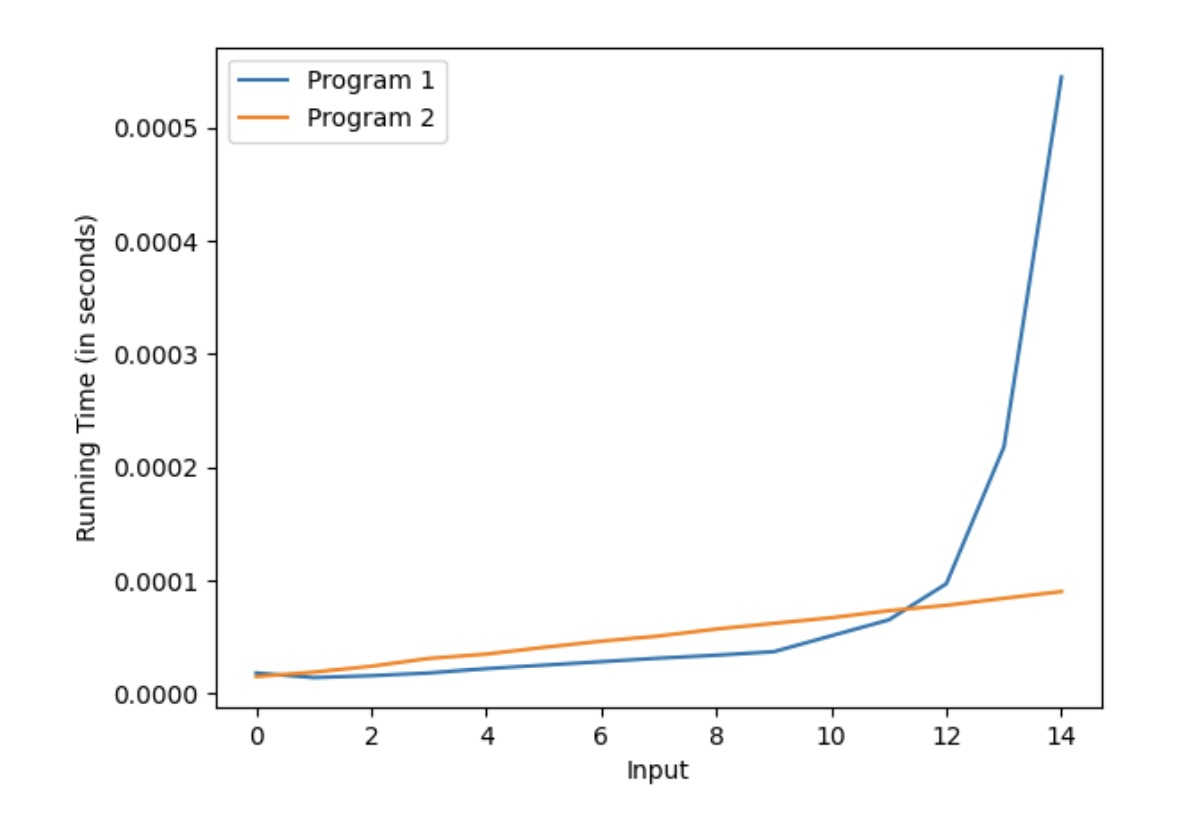
\includegraphics[scale = 0.5]{fall2024/psets/ps3/GraphCS120PS3.jpg}
    
    \item Explain the discrepancies you see between Parts~\ref{itm:RAMtime} and \ref{itm:realtime}.  (Hint: What do we know about the relationship between the RAM and Word-RAM models, and why is it relevant to how efficiently the Python simulation runs?) 
    \\\\ In part a, we said that both the algorithms run at linear runtime as the input size increases. However, in part b we can clearly see that Program 1 does not run linearly as input increases.
    \\ As for Program 2, the result is always reduced by a $\mod 2^{32}$ operation at each step, making sure that the output always stays fixed within a 32-bit range. Although we modeled it with the RAM model, this still fits the Word-RAM Model that Python actually runs on, where each word is of fixed size (32 or 64 bits), allowing arithmetic operations to be performed in $O(1)$ time. So, the runtime remains linear as expected.
    \\ But, Program 2 operates under the theoretical RAM model, which doesn't restrict the size of words. In reality, it lacks the modulus operation, and so the output grows exponentially with $N$. As $N$ increases, the result can exceep $2^{32}$, requiring multiple memory locations to store the value. If the output occupies $m = \frac{N}{32}$ with the ceiling function applied, meaning each arithmetic operation will take $O(m^2)$ time, significantly increasing runtime. So, the RAM model assumes constant-time operations, and the exponential growth of the output means that Program 1's actual runtime scales much worse than Program 2's as N grows larger. 
    
    \item (optional\footnote{This problem won't make a difference between N, L, R-, and R grades.}) Give a theoretical explanation of the shapes of the runtime curves you see in Part~\ref{itm:realtime}, by providing explicit formulas for the asymptotic runtimes of the two programs (in clock time). You may need to do some research online and/or make guesses about how Python operations are implemented to come up with your estimates. 

\end{enumerate}

\item (Simulating Word-RAM by RAM) For every Word-RAM program $P$, there is a RAM program $P'$ that simulates $P$ in the sense that:
\begin{enumerate}
    \item $P'$ halts on $(w,x)$ iff $P[w]$ halts on $x$, and 
    \item If $P[w]$ crashes, then $P'$ halts with $\outputpointer=\outputlen=0$. (We are using this output setting to indicate \crash, since the RAM model does not have any crashing in its semantics.)
    \item If $P[w](x)$ halts without crashing, then the output of $P'(x,w)$ equals the output of $P[w](x)$.
     Furthermore,   
       $$\Time_{P'}(x) = O\left(\Time_{P[w]}(x)+n+w\right),$$
where $n$ is the length of $x$.

(This was stated without proof in Lecture Notes 8.) \\
\end{enumerate}
To prove that for every Word-RAM program P, there exists a corresponding RAM program P' that simulates P while satisfying all conditions, we need to show how a RAM program handles all Word-RAM operations, including intialization, arithmetic, and other processes.
\begin{itemize}
    \item Initialization
    \\\\ Word-RAM is different from RAM in the way that it has a fixed word length $w$ and a memory size $S$, which is initially equal to $n$- the input array x's length. On the other hand, RAM has no fixed word length of memory limit, and is theoretical. Therefore, P' simulates this by calculating $S$ and $w$ from $x$, where $x$ is stored in memory locations $M[0],....,M[n-1]$, with all other locations being set to 0.
    \begin{itemize}
        \item Input Size Calculation: We iterate through the memory to determine the size $n$ of $x$, incrementing a counter until a memory location with value 0 is reached
        \item Word Length Calculation: Calculate $2^w$ by either exponentiation by squaring or by multiplying 2 by itself $w$ times.
    \end{itemize}
    If $S > 2^w$ or any element in $x$ exceeds $2^w-1$, the program crashes. This is how we uphold the Word-RAM model as for initialization.

    \item Operations
    \begin{itemize}
        \item Arithmetic (Addition, Multiplication): These operations are performed similar in RAM as they are in WOrd-RAM. However, the result must be checked to ensure that it is with the bounds (less than $2^w$). If the result exceeds $2^w$, we cap it at $2^w-1$.
        \item Subtraction and Division: These operations are unchanged between RAM and Word-RAM
        \item Memory Access (read/write): RAM simulates Word-RAM memory by ensuring that memory accesses do not exceed $2^w$. If an address is out of bounds, the program crashes.
        \item MALLOC: In Word-RAM, the MALLOC operation increases S by 1. In RAM, this is simulated by incrementing the input length. But, again, if $S > 2^w$, the program crashes.
        \item GOTO: GOTO operations are performed similarly in both models, though line numbers may change slightly due to additional checks in RAM.
        
    \end{itemize}
    \item Output and Crashing
    \\\\ The program crashes if any memory address or value exceeds $2^w-1$, or if $S \geq 2^w$. This is simulated in RAM by halting the program with $output-ptr = 0$ and $output-len = 0$. If no crash occurs, both programs halt with the same output.
    \item Runtime
    \\\\ The total runtime of $P'$ can be analyzed by considering three components:
    \begin{itemize}
        \item $O(n)$: Looping through the input array to determine its size takes $O(n)$, where $n$ is the length of $x$
        \item $O(w)$: Calculating $2^w$ in the iniatilization phase takes $O(w)$ steps.
        \item $T_{P[w]}(x)$: The runtime of the Word-RAM program is a subset of the RAM program's runtime, since all operations in RAM simulate those of Word-RAM with some constant overhead for boundary checks. 
    \end{itemize}
    So, the overall runtime of the RAM program is:
    \begin{equation*}
        T_{P'}(x) = O(T_{P[w]}(x) + n + w)
    \end{equation*}
    \item Conclusion
    \\\\ We have shown that the RAM program $P'(x,w)$ simulates the Word-RAM program $P[w](x)$ while preserving all operations and conditions, including handling memory, arithmetic, and crashes. The runtime of $P'$ is $(T_{P[w]}(x) + n + w)$, satisfying the conditions outlined. 
\end{itemize}

\item (reflection) Discuss the value (or lack thereof) that you think computational models, and the RAM and Word-RAM models in particular, have for computer science.  All opinions are valid, as long as they show serious thought and are backed by specific justifications.

\textit{Note: As with the previous psets, you may include your answer in your PDF submission, but the answer should ultimately go into a separate Gradescope submission form.}

\item Once you're done with this problem set, please fill out \href{https://forms.gle/TG8cG4LWN3S4T6za6}{this survey} so that we can gather students' thoughts on the problem set, and the class in general. It's not required, but we really appreciate all responses!

\end{enumerate}


\end{document}
